\documentclass[10pt]{article}

\usepackage{parskip}
\usepackage{amsmath}
\usepackage{physics}
\usepackage{natbib}
\usepackage{graphicx}

\title{Simple Land Surface Scheme}
\author{Tristan Abbott}
\date{\today}

\begin{document}

\maketitle

This land surface scheme solves equations for surface energy balance:
\begin{equation}
C_s \dv{T_s}{t} = Q_S - Q_L - H - L
\end{equation}
and the surface moisture balance
\begin{equation*}
\dv{W}{t} = P - E.
\end{equation*}
Expressing soil moisture $W$ in terms of a volumetric soil water content $\phi = W/D$, where $D$ is the soil depth, gives
\begin{equation}
\dv{\phi}{t} = \frac{P}{D} - \frac{E}{D}.
\end{equation}

Net longwave and shortwave fluxes must be computed externally and specified. The surface sensible heat flux $H$ and latent heat flux $L$ are parameterized (following \citet{RieckHoheneggerHeerwaarden2014}) as
\begin{equation} \label{eqn:H}
H = \frac{\rho c_p}{r_a} \qty (\theta_s - \theta_{\mathrm{atm}})
\end{equation}
and
\begin{equation} \label{eqn:S}
L = \frac{\rho L_v}{r_a + r_s} \qty [q^*(\theta_s) - q_{\mathrm{atm}}].
\end{equation}
The surface resistance $r_s$ is modeled (following \citet{HoheneggerStevens2018}) as a soil moisture dependent ramp
\begin{equation} \label{eqn:r_s}
r_s = r_s(\phi_{fc}) \frac{\phi_{fc} - \phi_{pwp}}{\phi - \phi_{pwp}}.
\end{equation}
The aerodynamic resistance $r_a$ is computed from the drag coefficient $C_k$ and near-surface wind speed $|{\bf u}_{\mathrm{atm}}|$ as
\begin{equation}
r_a = \frac{1}{C_k |{\bf u}_{\mathrm{atm}}|}.
\end{equation}
Finally, vertical momentum fluxes (i.e. surface stresses) are parameterized by a drag law
\begin{equation}
\tau_i = -C_d |{\bf u}_{\mathrm{atm}}| u_i.
\end{equation}

\section{Byun (1990) Monin-Obukhov scheme}

One option for modelling drag coefficients follows \citet{Byun1990}. The goal of the model is to relate surface fluxes of heat, momentum, and moisture to winds, temperature, and moisture at the surface and the lowest model level; i.e. to calculate
\begin{equation*}
C_d = \frac{u_*^2}{|{\bf u}_{\mathrm{atm}}|^2}
\end{equation*}
\begin{equation*}
C_H = \frac{\overline{w' \theta'}} {|{\bf u}_{\mathrm{atm}}| (\theta_s - \theta_{\mathrm{atm}})}
\end{equation*}
and
\begin{equation*}
C_L = \frac{\overline{w'q'}} {|{\bf u}_{\mathrm{atm}}| \qty [q^*(\theta_s) - q_{\mathrm{atm}}]}.
\end{equation*}
As a simplification, we will assume $C_L = C_H = C_k$ and calculate scalar drag coefficients using potential temperature fields. The first step in the formulation is to define a temperature scale based on the surface heat flux $\overline{w' \theta'}$ and the friction velocity $u_*$:
\begin{equation*}
\theta_* = \frac{\overline{w' \theta'}}{u_*}.
\end{equation*}
The Monin-Obukhov similarity hypothesis assumes that momentum and potential temperature profiles near the surface are described by nondimensional profile functions
\begin{equation*}
\frac{kz}{u_*} \pdv{u}{z} = \gamma_m \qty(\zeta)
\end{equation*}
and
\begin{equation*}
\frac{kz}{\theta_*}\pdv{\theta}{z} = \gamma_h \qty(\zeta),
\end{equation*}
where $k = 0.4$ is the von Karman constant. Common observation-based forms for the profile functions \citep{BusingerEtAl1971} are
\[
\gamma_m = 
\begin{cases}
1 + \alpha_m \zeta & \zeta \ge 0 \\
\qty(1 - \beta_m \zeta)^{-1/4} & \zeta < 0
\end{cases}
\]
and
\[
\gamma_h = 
\begin{cases}
\mathrm{Pr}_0 (1 + \alpha_h \zeta) & \zeta \ge 0 \\
\mathrm{Pr}_0 (1 - \beta_h \zeta)^{-1/2} &  \zeta < 0
\end{cases}
\]
with $\mathrm{Pr}_0 = 0.74$, $\alpha_m = 4.7$, $\alpha_h = \alpha_m/\mathrm{Pr}_0$, $\beta_m = 15$, and $\beta_h = 9$. $\zeta$ is the Monin-Obukhov stability parameter
\begin{equation*}
\zeta = \frac{z}{L} = \frac{k z g \theta_*}{\theta_s u_*^2}.
\end{equation*}
This parameter is closely related to the gradient Richardson number, which expressed in terms of the profile functions is
\begin{equation*}
\mathrm{Ri} = \frac{g}{\theta_s} \frac{\partial \theta / \partial z}{\qty(\partial u / \partial z)^2} = \zeta \frac{\gamma_h}{\gamma_m^2}.
\end{equation*}
However, because we have temperatures and velocities only at the surface and the lowest model level, we would prefer to relate $\zeta$ to the bulk Richardson number
\begin{equation} \label{eqn:Ri_b}
Ri_b = \frac{g}{\theta_s}\frac{(\theta_{\mathrm{atm}} - \theta_s)(z_{\mathrm{atm}} - z_s)}{|{\bf u}(z)|^2}.
\end{equation}

$\zeta$ can be expressed in terms of the bulk Richardson number using integrals of the profile functions from a surface roughness length $z_0$ to $z_{\mathrm{atm}}$. (Details are in \citet{Byun1990}.) Under stable conditions ($\zeta, \mathrm{Ri}_b \ge 0$),
\begin{align} 
\zeta &= \frac{1}{2 \alpha_h (\alpha_m \mathrm{Ri}_b - 1)} \qty[ -(2 \alpha_h \mathrm{Ri}_b - 1) - \qty(1 + \frac{4(\alpha_h - \alpha_m) \mathrm{Ri}_b}{\mathrm{Pr}_0})^{1/2} ] \\
&= \label{eqn:zeta1} \frac{\qty(\frac{z}{z - z_0}) \ln \qty(\frac{z}{z_0})}{2 \alpha_h (\alpha_m \mathrm{Ri}_b - 1)} \qty[ -(2 \alpha_h \mathrm{Ri}_b - 1) - \qty(1 + \frac{4(\alpha_h - \alpha_m) \mathrm{Ri}_b}{\mathrm{Pr}_0})^{1/2} ].
\end{align}
Under unstable conditions ($\zeta, \mathrm{Ri}_b < 0$), expressing $\zeta$ in terms of the bulk Richardson number is difficult, but a very good approximate solution can be found by multiplying an expression for $\zeta$ in terms of the gradient Richardson number by $\frac{z}{z - z_0} \ln \qty(\frac{z}{z_0})$ and replacing $\mathrm{Ri}$ with $\mathrm{Ri}_b$. This gives
\begin{equation} \label{eqn:zeta2}
\zeta = 
\begin{cases}
\frac{z}{z - z_0} \ln \qty(\frac{z}{z_0}) \qty [ -2 \sqrt{Q_b} \cos \qty(\frac{\theta_b}{3}) + \frac{1}{3 \beta_m}] & \mathrm{Ri}_b \le -0.2097 \\
\frac{z}{z - z_0} \ln \qty(\frac{z}{z_0}) \qty [-\qty(T_b + \frac{Q_b}{T_b}) + \frac{1}{3 \gamma_m}] & -0.2097 < \mathrm{Ri}_b \le 0.
\end{cases}
\end{equation}
with
\begin{align*}
s_b &= \frac{\mathrm{Ri}_b}{\mathrm{Pr}_0} \\
Q_b &= \frac{1}{9} \qty [\frac{1}{\beta_m^2} + 3 \frac{\beta_h}{\beta_m} s_b^2] \\
P_b &= \frac{1}{54} \qty [-\frac{2}{\beta_m^3} + \frac{9}{\beta_m} \qty(-\frac{\beta_h}{\beta_m} + 3) s_b^2] \\
\theta_b &= \acos \qty [\frac{P_b}{Q_b^{3/2}}] \\
T_b &= \qty [ \qty(P_b^2 - Q_b^3)^{1/2} + |P_b|]^{1/3}.
\end{align*}

Relationships between $u_*$, $\theta_*$, and resolved temperature and velocity fields can be derived from integrals of the profile functions:
\begin{equation*}
u_* =k |{\bf u}_{\mathrm{atm}}| \qty[\ln \qty(\frac{z}{z_0}) - \psi_m]^{-1},
\end{equation*}
and
\begin{equation*}
\theta_* = \frac{k \qty(\theta_{s} - \theta_{\mathrm{atm}})}{\mathrm{Pr}_0} \qty[\ln \qty(\frac{z}{z_0}) - \psi_h]^{-1}.
\end{equation*}
For stable conditions,
\begin{equation*}
\psi_m = -\alpha_m \zeta \qty(1 - \frac{z_0}{z})
\end{equation*}
and
\begin{equation*}
\psi_h = -\alpha_h \zeta \qty(1 - \frac{z_0}{z}).
\end{equation*}
For unstable conditions,
\begin{equation*}
\psi_m = 2 \ln \qty(\frac{1 + x}{1 + x_0}) + \ln \qty(\frac{1 + x^2}{1 + x_0^2}) - 2 \atan \qty(x) + 2 \atan \qty (x_0)
\end{equation*}
and
\begin{equation*}
\psi_h = 2 \ln \qty (\frac{1 + y}{1 + y_0})
\end{equation*}
with
\begin{align*}
x &= \qty[1 - \beta_m \zeta]^{1/4} \\
x_0 &= \qty[1 - \beta_m \zeta \frac{z_0}{z}]^{1/4} \\
y &= [1 - \beta_h \zeta]^{1/2} \\
y_0 &= [q - \beta_h \zeta \frac{z_0}{z}]^{1/2}.
\end{align*}

Combining these expressions with expressions for the surface drag law gives
\begin{equation} \label{eqn:tau_i}
\tau_i = -k^2 \qty[\ln\qty(\frac{z}{z_0}) - \psi_m]^{-2} |{\bf u}_{\mathrm{atm}}| u_{\mathrm{atm},i}.
\end{equation}
Similarly, the surface aerodynamic resistance $r_a$ is given by
\begin{equation} \label{eqn:r_a}
r_a = \frac{\mathrm{Pr}_0 \qty[\ln \qty(\frac{z}{z_0}) - \psi_m] \qty[\ln \qty(\frac{z}{z_0}) - \psi_h]}{k^2 |{\bf u}_{\mathrm{atm}}|}.
\end{equation}

The algorithm for computing surface fluxes is as follows
\begin{enumerate}
\item Calculate $Ri_b$ using Equation \ref{eqn:Ri_b}
\item Calculate $\zeta$ using Equation \ref{eqn:zeta1} or \ref{eqn:zeta2}
\item Calculate $\tau_i$ using Equation \ref{eqn:tau_i} and $r_a$ using Equation \ref{eqn:r_a}
\item Calculate $r_s$ from Equation \ref{eqn:r_s}
\item Calculate $H$ and $S$ from Equations \ref{eqn:H} and \ref{eqn:S}
\end{enumerate}

\subsection{Results}

Surface exchange and drag coefficients increase as the boundary layer becomes increasingly unstable (Figure \ref{fig:Byun4}). For stable boundary layers, exchange coefficients are set to zero above a critical bulk Richardson number of 0.21. Shutting turbulence off completely can have a dramatic impact on simulations run with a diurnal cycle over low heat capacity surfaces: these simulations frequently form nighttime radiation fog In the total absence of a nighttime atmosphere-to-surface moisture flux, but even a very small  moisture flux (on the order of 1 W/m$^2$) can be enough to prevent fog from forming.

\begin{figure}
\begin{center}
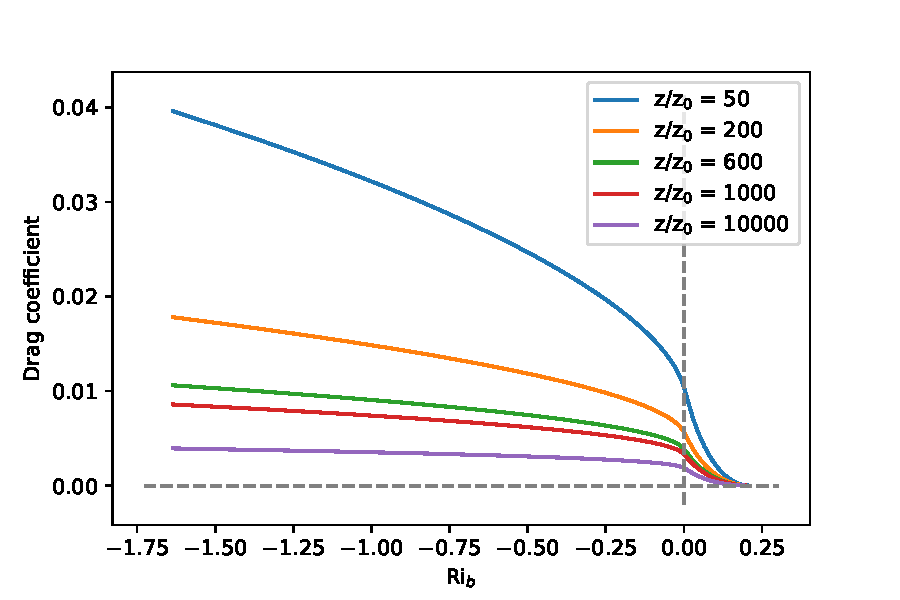
\includegraphics[height=0.4\textheight]{Byun1990Figure4a.pdf}
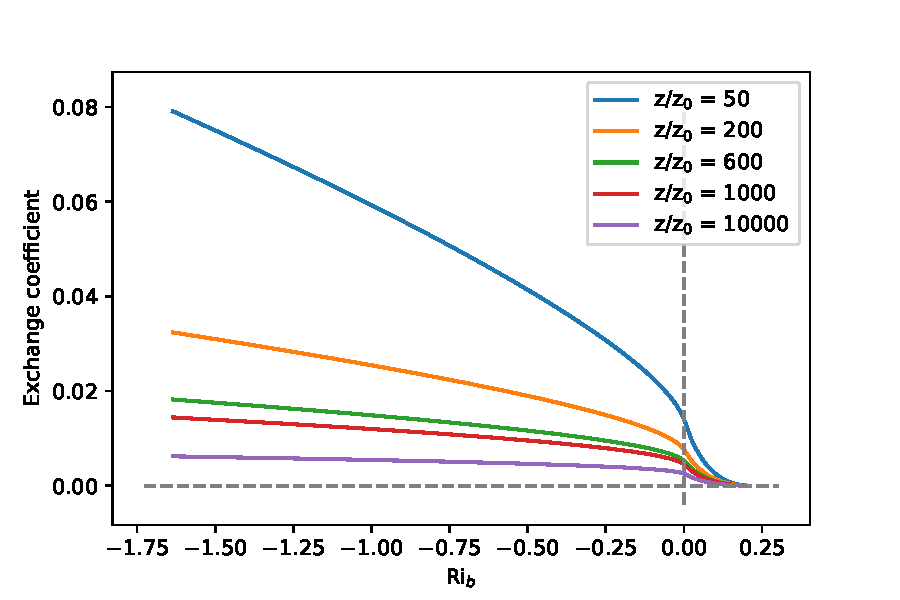
\includegraphics[height=0.4\textheight]{Byun1990Figure4b.pdf}
\end{center}
\caption{Variation of drag and exchange coefficients with bulk Richardson number for different surface layer depths.}
\label{fig:Byun4}
\end{figure}

\section{UCLA LES Monin-Obukhov scheme}

This land surface scheme also includes an option to model drag and exchange coefficients using profile functions from the UCLA LES \citep{Stevens2010}:
\[
\gamma_m = 
\begin{cases}
1 + \alpha_m \zeta & \zeta \ge 0 \\
\qty(1 - \beta_m \zeta)^{-1/2} & \zeta < 0
\end{cases}
\]
and
\[
\gamma_h = 
\begin{cases}
\mathrm{Pr}_0 (1 + \alpha_h \zeta) & \zeta \ge 0 \\
\mathrm{Pr}_0 (1 - \beta_h \zeta)^{-1/2} &  \zeta < 0
\end{cases}
\]
with $Pr_0 = 0.74$, $\alpha_m = 4.8$, $\alpha_h = 7.8$, $\beta_m = 19.3$, and $\beta_h = 12.0$.

\end{document}